\begin{frame}[noframenumbering,plain]
    \setcounter{framenumber}{1}
    \maketitle
\end{frame}


\begin{frame}
    \frametitle{Цели диссертации}
Целью данной работы является определение закономерностей, влияющих на перенос знаний между языками и задачами в многозадачных нейросетевых моделях на различных архитектурах и на особенности прикладного применения этих моделей в диалоговых платформах.

Для достижения этой цели требовалось решить следующие задачи:
\end{frame}

\begin{frame}
\frametitle{Задачи диссертации}
\begin{enumerate}
  \item {Определить закономерности переноса знаний при псевдоразметке данных для многозадачных нейросетевых моделей с одним линейным слоем.}
  \item {Определить закономерности переноса знаний в трансформер-инвариантных многозадачных нейросетевых моделях между различными диалоговыми задачами. Провести оценку зависимости этого переноса от размера обучающей выборки.}
  \item {Определить закономерности переноса знаний в многоязычных трансформер-инвариантных многозадачных нейросетевых моделях между различными языками -- с английского языка на русский. Провести оценку зависимости этого переноса от размера обучающей выборки. Рассмотреть применимость этих выводов для однозадачных моделей.}
  \item {Проверить зависимость межъязыкового переноса знаний на разговорных данных в многоязычных нейросетевых моделях от размера предобучающей выборки и генеалогической близости языков к языку дообучения.}
\end{enumerate}
\end{frame}

\begin{frame}
\frametitle{Задачи диссертации}
\begin{enumerate}
  \item {Разработать диалоговую платформу, задачи которой пригодны для изучения прикладного применения многозадачных моделей.} % TODO СПРОСИТЬ У ВАСИ
  \item {Интегрировать рассмотренные в диссертации многозадачные нейросетевые архитектуры в диалоговую платформу, оценить применимость данных архитектур и провести их сравнительный анализ на основе опыта практического применения. На основании этого анализа произвести интеграцию данных архитектур также в open-source библиотеку для решения задач машинного обучения.}% todo программную библиотеку
\end{enumerate}
\end{frame}




\begin{frame}
\frametitle{Оглавление}
\begin{enumerate}
    \item "Нейросетевые методы машинного обучения для задач обработки естественного языка"
    \item "Использование псевдоразметки данных в многозадачных моделях для решения задач GLUE"
    \item "Трансформер-инвариантные модели"
    \item "Исследование переноса знаний в многоязычных моделях на новом тематическом наборе данных"
    \item "Диалоговая платформа DREAM"
    \item " Использование в диалоговой платформе {DREAM} многозадачных моделей"
\end{enumerate}
\end{frame}

\begin{frame}{Первая глава}
Вводятся базовые понятия глубокого обучения. В частности, поясняется принцип работы модели BERT и разбираются многозадачные архитектуры на её основе - PAL-BERT и MT-DNN.
\end{frame}

\begin{frame}{Псевдоразметка данных: задача}
Определить закономерности переноса знаний при псевдоразметке данных для многозадачных нейросетевых моделей с одним линейным слоем.
\end{frame}
\begin{frame}{Псевдоразметка данных}
    Исследуются разные способы псевдоразметки данных при обучении BERT на следующих задачах из бенчмарка GLUE:
    \begin{enumerate}
    \item QQP -- задача классификации пар предложений из сайта Quora.com на 2 класса -- и не дубликат.
    \item MNLI -- задача классификации пар предложений из различных тем на три класса -- логическое следование, логическое противоречие и нейтральный(ни следование, ни 
    -- из тех же тем, что и тренировочный(MNLI-matched) и из остальных тем (MNLI-mismatched).
    \item SST-2 -- задача классификации предложений на два класса -- положительная тональность и отрицательная тональность.
    \item RTE -- задача классификации пар предложений на два класса -- логическое следствие и нет логического следствия.
    \end{enumerate}
\end{frame}


\begin{frame}{Способы псевдоразметки данных}
    \begin{enumerate}
\item Базовый способ -- стандартное обучение однозадачных моделей.
\item Независимые метки -- метки для каждой задачи считаются независимыми (т.е всего девять классов), каждый пример имеет метку 1 для того класса своей задачи, к которому он принадлежит и 0 для всех остальных классов всех остальных задач. 
\item Независимые метки, замороженная голова -- аналогично режиму Независимые метки, но линейный слой заморожен и обучается только тело модели.
\item Мягкие независимые метки -- аналогично предыдущему подходу, но вероятности всех остальных классов каждой из остальных задач считаются равными друг другу так, чтобы их сумма равнялась 1. 
\item Мягкие независимые метки, замороженная голова -- аналогично режиму Мягкие независимые метки, но линейный слой заморожен и обучается только тело модели.
    \end{enumerate}
\end{frame}


\begin{frame}{Способы псевдоразметки данных}
    \begin{enumerate}
\item Дополненные независимые метки -- аналогичен режиму Мягкие независимые метки, но вероятности для всех классов каждой из остальных задач получаются при помощи предсказаний однозадачной модели, обученной исключительно на этой задаче.
\item Мягкое вероятностное предположение -- объединение классов с сокращением их числа до пяти: положительный, отрицательный, логическое следствие, логическое противоречие, нейтральный. В остальном та же логика, что и для режима Мягкие независимые метки.
\item Мягкие предсказанные метки -- аналогичен предыдущему, но все недостающие вероятности для каждой из задач не считаются равновероятными, а определяются дополнительной разметкой от модели для каждой задачи. 
\item Жесткие предсказанные метки -- аналогичен предыдущему, но для меток, полученных из предсказаний оригинальной модели, максимальная вероятность для каждой задачи округляется до 1, а все остальные вероятности до 0.
    \end{enumerate}
\end{frame}

\begin{frame}{Псевдоразметка данных: результаты}
\begin{table}[htbp]
\centering
\caption {Лучшая точность на тестовых данных (при лучшей скорости обучения из выбираемых, среднее по 3 запускам)}
\label{tab:ps2}% label всегда желательно идти после caption
\resizebox{\textwidth}{!}
{%
\begin{tabular}{|c||c|c|c|c|c|c|}
\hline
\multirow{2}{*}{Эксперимент} & \multicolumn{6}{c|}{Задача}  \\
\cline{2-7}
& Среднее& RTE& QQP& MNLI-m &MNLI-mm& SST-2\\
\hline
Базовый (оригинальная статья) & 78.8 & 66.4  & 71.2 & 84.6 & 83.4 & 93.5 \\
\hline
Базовый (воспроизведённый) & 77.6 & 62.7 & 71.0 & 83.1 & 82.7 & 93.5 \\
\hline
Независимые метки &79.0 & 71.5 & 70.9 & 82.7 & 81.7 & 91.3 \\
\hline
Мягкие независимые метки  &78.9 & 69.3 & 71.3 & 82.8 & 82.1 & 92.6 \\
\hline
Дополненные независимые метки &77.6 & 64.2&\textbf{ 71.8} & 81.2 & 80.7 & \textbf{93.2} \\
\hline
Мягкое вероятностное предположение  &\textbf{79.7} & \textbf{72.7} & 70.7 &\textbf{ 83.4} &\textbf{82.3} & 92.5 \\
\hline
Мягкие предсказанные метки  & 78.8 & 70.3 & 70.7 & 81.7 & 81.7 & 92.5 \\
\hline
Жесткие предсказанные метки & 79.1 & 71.3 &71.1 & 81.7 & 81.4 & 92.6 \\
\hline
\begin{tabular}[c]{@{}l@{}}Независимые метки,\\замороженная голова\end{tabular}   & 78.2 & 66.9& \textbf{71.8} & 82.6 & 81.8 & 91.9 \\
\hline
\begin{tabular}[c]{@{}l@{}}Мягкие независимые метки,\\замороженная голова\end{tabular}  &79.1 & 70.0 & 71.5 & 83.0 &\textbf{ 82.3} & 92.4 \\
\hline
\end{tabular}
}
\end{table}
\end{frame}

\begin{frame}{Псевдоразметка данных: выводы}
\begin{enumerate}
\item На задачах, сильнее всего похожих друг на друга (MNLI и RTE) лучше всего показывают себя способы, подразумевающие объединение меток, что говорит о том, что в определенных случаях оно может быть оправдано. 

\item С другой стороны, объединение меток не даёт улучшений для более разнородных задач, таких, как QQP и SST, что показывает ограничения этого метода. Лучше всего для таких задач показывает себя метод Дополненные независимые метки, подразумевающий параллельную псевдоразметку данных. 

\item Главный вывод из этой главы -- псевдоразметка данных при помощи однозадачных моделей улучшает метрики многозадачных моделей. При этом объединение классов оправдывает себя только для задач, достаточно сильно похожих друг на друга. 
\end{enumerate}
\end{frame}

\begin{frame}{Трансформер-инвариантные модели: задача}
\begin{enumerate}
    \item Определить закономерности переноса знаний в трансформер-инвариантных многозадачных нейросетевых моделях между различными диалоговыми задачами. 
    \item Провести оценку зависимости этого переноса от размера обучающей выборки.
 \end{enumerate}
\end{frame}

\begin{frame}{Трансформер-инвариантные модели: архитектура}
\begin{itemize}

  \item Как и в оригинальной статье~\cite{bert}, возвращаются финальные скрытые состояния для всех токенов и выход пулингового слоя базовой модели-трансформера. 
  
  \item К выходу пулера применяется дропаут, по умолчанию равный 0.2. Для задач выбора из нескольких вариантов ответа или классификации каждого токена в предложении, выход преобразуется аналогично соответствующим задачам.

  \item После этого этапа, применяется задаче-специфичный линейный слой с размерностью выхода {n}. Для всех задач, кроме регрессии или выбора из нескольких вариантов ответа, \footnote{Для задачи выбора из нескольких вариантов ответа, каждой метке изначально относится несколько примеров. Т.е с таким числом классов после преобразования формы число реальных и предсказанных меток соответствует друг другу.} {n} равняется числу классов для задачи. Во всех других случаях {n} равняется 1.
 
  \item В конце применяется функция потерь. Если для каждого примера из задачи ожидается только одна метка, применяется категорическая кросс-энтропия, в остальных случаях -- бинарная кросс-энтропия. 

\end{itemize}
\end{frame}

\begin{frame}{Трансформер-инвариантные модели: достоинства архитектуры}
\begin{itemize}

  \item Вычислительная и архитектурная простота
  \item Расширяемость на различные типы задач
  \item Не требует псевдоразметки

\end{itemize}
\end{frame}

\begin{frame}{Трансформер-инвариантные модели: принцип подбора данных}
\begin{itemize}
    \item Разговорные задачи
    \item Совпадающие классы для английского и русского языка
\end{itemize}
\end{frame}

\begin{frame}{Трансформер-инвариантные модели: данные}
\begin{itemize}
    \item Для классификации эмоций -- русскоязычный набор данных CEDR, собранный из различных интернет-источников, и англоязычный набор данных go\_emotions, собранный из комментариев на ресурсе «Реддит». Использовалось семь типов эмоций по Экману -- ярость, страх, грусть, удовольствие, удивление, отвращение, нейтральная.
    \item Для классификации тональности -- англоязычный набор данных DynaSent(r1), состоящий из предложений, возникающих в диалогах, и русскоязычный набор данных RuReviews, состоящий из отзывов крупного российского электронного магазина. Использовалось три класса -- положительный, отрицательный, нейтральный.
\end{itemize}
\end{frame}

\begin{frame}{Трансформер-инвариантные модели: данные}
\begin{itemize}
    \item Для классификации токсичности -- русскоязычный набор комментариев с ресурса «Двач» (RuToxic) и англоязычный набор комментариев из Википедии (Wiki Talk). Использовалось два класса -- токсичный и не токсичный.
    \item Для классификации тем и классификации интентов -- набор данных MASSIVE, состоящий из обращенных к диалоговой системе фраз пользователей. Набор существует и использовался как в англоязычном, так и в русскоязычном варианте. Каждая фраза из набора принадлежит к одной из 60 тем и к одному из 18 интентов.
\end{itemize}
\end{frame}

\begin{frame}{Трансформер-инвариантные модели: сравнение с однозадачными}
\begin{table}[htbp]
\centering
\caption {Метрики англоязычных моделей (точность/макро-F1) для пяти англоязычных диалоговых задач.Режим S означает однозадачные модели, режим M означает многозадачные модели. Усреднено по трем запускам.}
\scalebox{1}{
\begin{tabular}{|c|c|c|c|c|c|c|c|}
\hline
\multirow{2}{*}{Модель} & \multirow{2}{*}{Режим} & \multirow{2}{*}{Среднее} & Эмоции & Тональность & Токсичность & Интенты & Темы \\
& & & 39.4k & 80.5k & 127.6k & 11.5k & 11.5k \\ \hline \hline
\textit{\multirow{2}{*}{distilbert}} & S & \textbf{82.9} & \textbf{70.3} & 74.7 & 91.5 & \textbf{87.4} & \textbf{91.0} \\ %\hline
 & M  & 82.1 & 67.7 & \textbf{75.2} & 90.6 & 86.3 & 90.8  \\ \hline
\textit{\multirow{2}{*}{bert}} & S & \textbf{83.9} & \textbf{71.2} & 76.1 & \textbf{93.2} & \textbf{87.9} & \textbf{91.3} \\ %\hline
 & M &  83.0 & 69.0 & \textbf{76.5} & 91.4 & 87.1 & 91.2 \\ \hline
\textit{\multirow{2}{*}{bert}} & S & \textbf{84.7} & \textbf{70.9} & \textbf{80.5} & \textbf{92.1} & \textbf{88.4} & 91.3 \\ %\hline
 & M  & 83.6 & 69.0 & 79.0 & 91.3 & 87.3 & \textbf{91.3} \\ \hline
 \end{tabular}}
 \end{table}
 \end{frame}
 \begin{frame}
\begin{table}[htbp]
\centering
\caption {Метрики русскоязычных моделей (точность/f1 macro) для пяти диалоговых задач. Режим S означает однозадачные модели, режим M означает многозадачные модели. Усреднено по трем запускам.} 
\scalebox{1}{
\begin{tabular}{|c|c|c|c|c|c|c|c|}
\hline
\multirow{2}{*}{Модель} & \multirow{2}{*}{Режим} & \multirow{2}{*}{Среднее} & Эмоции & Тональность & Токсичность & Интенты & Темы \\
& & & 6.5k & 82.6k & 93.3k & 11.5k & 11.5k \\ \hline \hline
\textit{\multirow{2}{*}{distilrubert}} & S & 86.9 & 82.2 & 77.9 & 97.1 & 86.7 & 90.4  \\
 & M & 86.3 & 81.0 & 77.7 & 96.9 & 85.2 & 90.7 \\ \hline
\textit{\multirow{2}{*}{rubert}} & S & 86.5 & 80.9 & 78.0 & 97.2 & 86.2 & 90.0  \\ 
 & M & 86.2 & 80.5 & 77.6 & 96.8 & 85.3 & 90.5 \\ \hline
 \end{tabular}}
 \end{table}
 

\end{frame}

\begin{frame}
\begin{table}{htbp}
\caption{Трансформер-инвариантные модели: результаты на GLUE}
%\resizebox{\textwidth}{!}
\scalebox{0.52}{
\begin{tabular}{|c|c|c|c|c|c|c|c|c|c|c|c|}
\hline
\multirow{3}{*}{Модель} & \multirow{3}{*}{Режим}  & Среднее & CoLA & SST-2 & MRPC &STS-B &QQP&MNLI & QNLI & RTE & AX  \\
\cline{3-11}
   &  & Размер  & 8.6k & 67.3k & 2.5k & 5.7k & 363.8k & 392.7k & 104.7k & 2.5k & как у MNLI  \\ 
\cline{3-11}   
   &  & метрика  & M.Corr & Acc & F1/Acc & P/S Corr & F1/Acc & Acc (m/mm) & Acc & Acc & M.Corr \\ \hline \hline
Человек & - & 87.1 & 66.4 & 97.8 & 86.3/80.8 & 92.7/92.6 & 59.5/80.4 & 92.0/92.8 & 91.2 & 93.6 & - \\ \hline
\textit{\multirow{2}{*}{distilbert}} & S & 73.3 & \textbf{42.4} & \textbf{92.1} & 85.6/\textbf{80.3} & 78.8/76.8 & \textbf{69.5/88.5} & \textbf{81.3/80.8} & \textbf{87.5} & 52.1 & 29.9  \\ 
 & M & \textbf{74.5} & 36.0 & 91.0 & \textbf{85.7}/79.9 & \textbf{82.6/81.6} & 68.4/87.4 & 80.4/80.3 & 86.0 & \textbf{69.5} & \textbf{30.1} \\  \hline
\textit{\multirow{2}{*}{bert}} & S & 77.3 & \textbf{53.7} & \textbf{93.2} & \textbf{87.7/82.8} & 83.8/82.2 & \textbf{70.3/88.9} & \textbf{83.8/83.1} & \textbf{90.6} & 62.1 & 32.1 \\ 
 & M & \textbf{77.8} & 45.8 & 92.9 & 86.8/82.2 & \textbf{85.3/84.7} & 70.2/88.6 & 83.5/82.6 & 90.1 & \textbf{74.5} & \textbf{32.8} \\  \hline
\textit{\multirow{2}{*}{bert-large}} & S & \textbf{79.5} & \textbf{59.2} & \textbf{94.9} & 85.0/80.6 & \textbf{85.8/84.5} & 70.5/89.1 & \textbf{86.7/85.6} & 92.2 & 70.1 & \textbf{39.4} \\ 
 & M & \textbf{79.5} & 50.8 & 94.1 & \textbf{87.3/82.8} & 83.8/83.9 & \textbf{71.0/89.2} & 85.9/85.0 & \textbf{92.4} & \textbf{78.5} & 38.5 \\  \hline
\end{tabular}}
\end{table}
%\end{table*}
\end{frame}

\begin{frame}{Трансформер-инвариантные модели: перенос знаний между языками}
%\resizebox{\textwidth}{!}
\scalebox{0.48}{
\begin{tabular}{|c|c|c||c|c|c|c|c|c|} \hline
Модель & \begin{tabular}[c]{@{}l@{}}Тренировочные\\данные\end{tabular} & Режим & Среднее & \begin{tabular}[c]{@{}l@{}}Эмоции\end{tabular} & \begin{tabular}[c]{@{}l@{}}Тональность\end{tabular} & \begin{tabular}[c]{@{}l@{}}Токсичность\end{tabular} & \begin{tabular}[c]{@{}l@{}}Интенты\end{tabular} & \begin{tabular}[c]{@{}l@{}}Темы\end{tabular} \\
\hline \hline
\textit{distilbert-mult} & RU & S & 84.7 & 77.4 & 77.7 & 96.7 & 83.5 & 88.1 \\ %\hline
\textit{distilbert-mult} & RU & M & 84.3 & 78.1 & 76.8 & 96.5 & 81.9 & 88.2  \\ \hline
\textit{distilbert-mult} & \begin{tabular}[c]{@{}l@{}}RU+EN,\\объединенные\end{tabular} & S & 85.2 & 78.9 & 77.4 & 96.8 & 84.7 & 88.4 \\ %\hline
\textit{distilbert-mult} & \begin{tabular}[c]{@{}l@{}}RU+EN,\\объединенные\end{tabular} & M & 84.5 & 77.9 & 76.6 & 96.5 & 82.9 & 88.4 \\ \hline
\textit{distilbert-mult} & \begin{tabular}[c]{@{}l@{}}RU+EN,\\отдельные\end{tabular} & M & 84.4 & 77.6 & 76.8 & 96.5 & 82.4 & 88.3 \\ \hline
\textit{bert-mult} & RU & S & 84.7 & 76.6 & 77.8 & 96.9 & 83.9 & 88.4 \\ %\hline
\textit{bert-mult} & RU & M & 84.8 & 78.4 & 76.3 & 96.8 & 83.7 & 89.0 \\ \hline
\textit{bert-mult} & \begin{tabular}[c]{@{}l@{}}RU+EN,\\объединенные\end{tabular} & S & 85.6 & 78.9 & 77.6 & 96.9 & 85.0 & 89.4 \\ %\hline
\textit{bert-mult} & \begin{tabular}[c]{@{}l@{}}RU+EN,\\объединенные\end{tabular} & M & 85.2 & 79.2 & 76.4 & 96.7 & 84.3 & 89.4 \\ \hline
\textit{bert-mult} & \begin{tabular}[c]{@{}l@{}}RU+EN,\\отдельные\end{tabular} & M & 85.0 & 78.3 & 77.1 & 96.7 & 84.0 & 89.1 \\ \hline
\end{tabular}}

\end{frame}


\begin{frame}{Трансформер-инвариантные модели - эффект уменьшения размера выборки}
\label{fig:thresholds_acc_ru}
\begin{minipage}{0.5\textwidth}
\begin{tikzpicture}[baseline={(0,2.1)}]%[scale=2]
\begin{axis}[xlabel = RU доля,
ylabel = Средняя точность,
legend pos= south east,
width=0.9\textwidth,
xtick={0,1,2,3,4,5,6,7,8},
xticklabels={2,3,5,10,15,20,25,50,100},
ymin=50,ymax=90,
legend cell align={left},
legend style={nodes={scale=0.5, transform shape}}
]
\addplot[color=orange,dotted, mark=*] coordinates {
(1, 57.02)
(2, 58.379999999999995)
(3, 75.66666666666667)
(4, 77.7)
(5, 78.36666666666667)
(6, 79.53333333333333)
(7, 82.5)
(8, 84.39999999999999)
};
\addlegendentry{S точность (RU)}
\addplot[color=red,solid,mark=*] coordinates {
(1, 65.88)
(2, 70.3)
(3, 75.23333333333333)
(4, 77.23333333333333)
(5, 79.0)
(6, 79.60000000000001)
(7, 82.3)
(8, 84.33333333333333)
};
\addlegendentry{M точность (RU)}
\addplot[color=cyan,dashed, mark=*] coordinates {
(1, 70.73333333333333)
(2, 74.23333333333333)
(3, 77.39999999999999)
(4, 78.89999999999999)
(5, 80.13333333333334)
(6, 80.93333333333332)
(7, 82.83333333333333)
(8, 84.36666666666667)
};
\addlegendentry{S точность (RU+EN)}
\addplot[color=blue,dashed,mark=*] coordinates {
(1, 71.8)
(2, 74.96666666666667)
(3, 77.93333333333334)
(4, 79.66666666666667)
(5, 80.56666666666666)
(6, 81.36666666666666)
(7, 83.23333333333333)
(8, 85.16666666666667)
};
\addlegendentry{M точность (RU+EN)}
\end{axis}%
\end{tikzpicture}
% \hspace{3mm}
% \captionof{figure}
% \caption{Av}
\end{minipage}
\begin{minipage}{0.5\textwidth}
\scalebox{0.7}{
\begin{tabular}[baseline={(0,2.1)}]{|l||c|c|c|c|}
\hline
RU & S & M & S & M \\
доля & RU & RU & RU+EN & RU+EN \\ % Sizes are different for RU and RU+EN, so I don't give them here
\hline
3 & 57.0 & \textbf{65.9} & \textbf{71.8} & 70.7 \\ 
% \hline
5 & 58.4 & \textbf{70.3} & \textbf{75.0} & 74.2\\ 
% \hline
10 & \textbf{75.7} & 75.2 & \textbf{77.9} & 77.4\\ 
% \hline
15 & \textbf{77.7} & 77.2 & \textbf{79.7} & 78.9\\ 
% \hline
20 & 78.4 & \textbf{79.0} & \textbf{80.6} & 80.1 \\ 
% \hline
25 & 79.5 & \textbf{79.6} & \textbf{81.4} & 80.9 \\ 
% \hline
50 & \textbf{82.5} & 82.3 & \textbf{83.2} & 82.8 \\ 
% \hline
100 & \textbf{84.4} & 84.3 & \textbf{85.2} & 84.4 \\ \hline
\end{tabular}}
\end{minipage}
\end{frame}

\begin{frame}{Трансформер-инвариантные модели - эффект уменьшения размера выборки, английские данные}
\scalebox{0.7}{
\begin{minipage}{0.5\textwidth}{
\begin{tikzpicture}
\label{fig:tr-ag:en_dialog_part}
\begin{axis}[xlabel = Процент используемых тренировочных данных,
ylabel = Средняя точность,
legend pos= south east,
% width=10cm,
% height=10cm,
% xmin=2,
% xmax=100,
xtick={2,3,5,7,9,10,15},
ymin=40,ymax=85,
legend cell align={left},
legend style={nodes={scale=0.7, transform shape}}
]
\addplot[color=blue,solid, mark=*] coordinates {
(2, 64.8)%50
(3, 68.8)%50
(5, 71.7)%100
(7,74.2)
%(7.5,74.6)
% (8,74.9)
(9,75.4)
(10, 75.9)%300
(15, 77.4)
};
\addlegendentry{Многозадачные модели}
\addplot[color=green,dashed,mark=*] coordinates {
(2, 44.9)%50
(3, 59.6)%100
(5, 69.1)%300
(7,73.5)
%(7.5,73.5)
% (8,73.8)%500
(9,76.7)
(10,77.1)
(15, 78.5)
};
\addlegendentry{Однозадачные модели}
\end{axis}%
\end{tikzpicture}}
\end{minipage}

\begin{minipage}{0.4\textwidth}
\scalebox{0.7}{
\begin{tabular}[baseline={(0,2.1)}]{|l||c|c|}
\hline
Доля & S & M \\ % Sizes are different for RU and RU+EN, so I don't give them here
\hline \hline
2 & 44.9 & 64.8 \\ \hline
3 & 59.6 & 68.8  \\ \hline
5 & 69.1 & 71.7 \\ \hline
7 & 73.5 & 74.2  \\ \hline
9 & 76.7 & 75.4  \\ \hline
10 & 77.1 & 75.9 \\ \hline
15 & 78.5 & 77.4  \\ \hline
\end{tabular}}
\end{minipage}
}
%
\end{frame}

\begin{frame}{Трансформер-инвариантные модели. Выводы.}
\begin{enumerate}
\item Многозадачные трансформер-инвариантные модели практически соответствуют однозадачным моделям по своим метрикам на диалоговых задачах. Для задач с недостаточно большими тренировочными наборами данных такие модели могут даже превосходить однозадачные модели по своей средней точности - за счет переноса знаний с задач, для которых тренировочных данных существенно больше. Обходясь при этом одним трансформером вместо нескольких.
\item Если для одной и той же задачи имеются обучающие данные для английского и для русского языка, соответствующие друг другу по номенклатуре и нумерации классов, эти данные при обучении трансформер-инвариантной многозадачной модели лучше использовать в рамках одной задачи, а не в рамках отдельной задачи для каждого языка. Это связано с тем, что при использовании данных из разных языков в рамках одной задачи перенос знаний происходит как на уровне тела модели, так и на уровне задаче-специфичных линейных слоев, тогда как если выделять данные для каждого языка в отдельную задачу, то перенос знаний между ними будет происходить только на уровне тела модели.
\end{enumerate}
\end{frame}
\begin{frame}{Трансформер-инвариантные модели. Выводы.}
\begin{enumerate}
\item При обучении моделей на небольших долях тренировочных данных(примерно до 10 процентов) многозадачные модели превосходят однозадачные по средней точности.
\item Как правило, превосходство в точности для каждой из задач сильно зависит от размера набора данных -- чем меньше урезанный набор данных, тем выше преимущество многозадачных моделей. Исключением из этого правила является русскоязычная задача классификации эмоций -- вероятно, тут роль играет эффект переноса знаний с задачи классификации тональности.
\end{enumerate}
\end{frame}
\begin{frame}{Трансформер-инвариантные модели. Выводы.}
\begin{enumerate}
\item Добавление англоязычных тренировочных данных к русскоязычным улучшает метрики на русскоязычных тестовых данных. Чем меньше размер имеющихся русскоязычных тренировочных данных, тем сильнее повышается точность моделей от добавления англоязычных данных -- и выигрыш в точности может достигать нескольких процентов, если объем русскоязычных тренировочных данных достаточно маленький. Этот вывод справедлив как для однозадачных, так и для многозадачных моделей, и язык валидационных данных (английских или русских) не влиял на результаты экспериментов.
\end{enumerate}
\end{frame}

\begin{frame}{Многоязычный перенос знаний}
Требования к набору данных - 
\begin{enumerate}
\item {Разговорные данные, не слишком длинные примеры}
\item {Много разговорных классов}
\item {Не слишком мало примеров}
\item{Русский язык}
\end{enumerate}
\end{frame}

\begin{frame}{Многоязычный перенос знаний - источник данных}
Равноразмерные: 1 вопрос - 1 ответ - 1 метка.
\begin{table}[htbp]
\caption{Размеры набора данных {RuQTopics} по классу и части}
%\centering
Набор данных RuQTopics получен с сервиса Яндекс. Кью.
\scalebox{0.6}{
\begin{tabular}{|c||c|c|c|c|c|} \hline
\textbf{тип данных}  & \multicolumn{2}{c|}{\textbf{однометочные}} & \multicolumn{2}{c|}{\textbf{многометочные}} & \multirow{2}{*}{\textbf{равноразмерные}}\\
\cline{1-5}
\textbf{класс}  & \multicolumn{1}{c|}{все} & \multicolumn{1}{c|}{отвеченные} & \multicolumn{1}{c|}{все} & \multicolumn{1}{c|}{отвеченные} & \\\hline \hline
\textit{Размер набора данных} & 361650 & 266597 & 170930 & 137341 & 264786\\ \hline
\textit{Размер 6классового поднабора данных} & 18864 & 15912 & 27191 & 20569 & 15830 \\ \hline
\textit{Музыка} & 9514 & 5809 & 4456 & 3287 & 5797 \\ \hline
\textit{Еда, напитки и кулинария} & 5750 & 4758 & 14096 & 11084 & 4723 \\ \hline
\textit{Медиа и коммуникации} & 4505 & 2637 & 5577 & 3948 & 2619 \\ \hline
\textit{Транспорт} & 2435 & 1625 & 1933 & 1387 & 1613 \\ \hline
\textit{Новости} & 945 & 602 & 912 & 720 & 600\\ \hline
\textit{Погода} & 890 & 481 & 217 & 143 & 478 \\ \hline
\end{tabular}
}
\end{table}
\end{frame}


\begin{frame}{Многоязычный перенос знаний - тестирование данных}
\begin{table}[htbp]
\caption{Различные типы базовых моделей: ru (rubert от DeepPavlov), rutiny (rubert-tiny от DeepPavlov), rusber (rubert от Сбербанка) и mult (multilingual BERT от авторов статьи) обучались на 6 классах из набора данных RuQTopics, предобработанном различными методами ( Q - вопросы, A - ответы, Q [SEP] A - конкатенация вопросов и ответов) и тестировались на соответствующих классах из наборах данных MASSIVE.}
\scalebox{1}{
\begin{tabular}{|c|c||c|}
\hline
\multirow{2}{*}{\textbf{Модель}} & \multirow{2}{*}{\textbf{Режим}} &  \multicolumn{2}{c|}{\textbf{Все классы}}  \\ 
\cline{3}
& & Точность   \\ \hline
\textit{ru} &  \textbf{Q} & 85.0 \\ %\hline
\textit{rutiny} &  \textbf{Q} & 85.7 \\ %\hline
\textit{rusber} &  \textbf{Q} & 85.5 \\ %\hline
\textit{mult} &  \textbf{Q} & 80.8 \\ \hline
\textit{ru} &  \textbf{A} & 79.8 \\ %\hline
\textit{rutiny} &  \textbf{A} & 82.4 \\ %\hline
\textit{rusber} &  \textbf{A} & 82.6 \\ %\hline
\textit{mult} &  \textbf{A} & 74.5 \\ \hline
\textit{ru} &  \textbf{Q [SEP] A} & 85.4 \\ %\hline
\textit{rutiny} &  \textbf{Q [SEP] A} & 85.3 \\ %\hline
\textit{rusber} &  \textbf{Q [SEP] A} & 85.1 \\ %\hline
\textit{mult} &  \textbf{Q [SEP] A} & 80.0 \\ \hline
\end{tabular}
}
\end{table}


\end{frame}


\begin{frame}{Многоязычный перенос знаний - главные выводы из тестирования данных}
\begin{enumerate}
\item Модели, учившиеся только на ответах, показывают лучшие результаты, чем учившиеся только на вопросах, а учившиеся только на ответах. Это верно для всех рассмотренных базовых моделях, что доказывает: вопросы -- самый информативный элемент набора данных {RuQTopics}. 

\item Конкатенация вопросов к ответам не дает стойкого улучшения по сравнению с использованием только лишь вопросов. 

\item В общем и целом, все русскоязычные модели показывают похожие результаты, а многоязычная модель ожидаемо показывает результаты хуже, чем любая из русскоязычных. 

\item Все эти выводы также справедливы для экспериментов, в которых использовались все данные из части 1 набора данных {RuQTopics}, принадлежащие вышеупомянутым шести классам.
\end{enumerate}
\end{frame}


\begin{frame}{Многоязычный перенос знаний между всеми языками из MASSIVE}
% TODO COMPRESS N
\begin{minipage}{0.5\textwidth}
\begin{table}[htbp]
\caption{Метрики модели \textit{bert-base-multilingual-cased} на объединенном тестовом наборе данных {MASSIVE} для всех языков. Модель обучалась на версии \textbf{Q} набора данных {RuQTopics}. \textbf{Код} означает код языка(ISO 639-1), \textbf{N} означает число статей в Википедии на этом языке на 11 октября 2018 года, \textbf{Дист} означает лингвистическую дистанцию между этим языком и русским, посчитанную в соответствии с работой~\cite{lang_sim}. Усреднено по трем запускам.}
{
\scalebox{0.55}{
\begin{tabular}[baseline={(0,2.1)}]{|c|c|c|c|c|} \hline
\multirow{2}{*}{\textbf{Язык}}  & \multirow{2}{*}{\textbf{Код}} & \multirow{2}{*}{\textbf{Дист}} & \multirow{2}{*}{\textbf{N}}  &  \multicolumn{2}{c|}{\textbf{Метрики}} \\ %\hline
\cline{5}
& & & & Точность & Макро-F1 \\ \hline \hline
русский & ru & 0 & 1.5M & 80.8 & 79.8\\
китайский (Тайвань) & zh-TW & 92.2 & 1M & 79.6 \\
китайский & zh & 92.2 & 1M & 78.0 \\
английский & en & 60.3 & 5.7M & 75.2 \\
японский & ja & 93.3 & 1,1M & 72.4 \\
словенский & sl & 4.2 & 162K & 70.3 \\
шведский & sv & 59.5 & 3.8M & 70.2 \\
%малайский & ms & n/c & 321K & 68.9 \\
итальянский & it & 45.8 & 1.5M & 68.8 \\
индонезийский & id & 91.2 & 441K & 68.7 \\
нидерландский & nl & 64.6 & 1.9M & 68.7 \\
португальский & pt & 61.6 & 1M & 68.6 \\
испанский & es & 51.7 & 1.5M & 68.2 \\
датский & da & 66.2 & 240K & 67.8 \\
французский & fr & 61.0 & 2M & 65.5 \\
персидский & fa & 72.4 & 644K & 65.2 \\
турецкий & tr & 86.2 & 317K & 64.5 \\
вьетнамский & vi & 95.0 & 1.2M & 64.3 \\
норвежский букмол & nb & 67.2 & 495K & 64.3 \\
польский & pl & 5.1 & 1.3M & 64.2 \\
азербайджанский & az & 87.7 & 139K & 63.9 \\
каталанский & ca & 60.3 & 592K & 61.4 \\
венгерский & hu & 87.2 & 438K & 61.3 \\
иврит & he & 88.9 & 232K & 60.9 \\
хинди & hi & 69.8 & 127K & 60.7 \\
корейский & ko & 89.5 & 429K & 60.4 \\
\hline
\end{tabular}
}
}
\end{table}
\end{minipage}
\end{frame}

\begin{frame}{Многоязычный перенос знаний между всеми языками из MASSIVE}
% TODO UPDATE ALL RUNS
\begin{minipage}{0.5\textwidth}
\begin{table}[htbp]
\caption{Метрики модели \textit{bert-base-multilingual-cased} на объединенном тестовом наборе данных {MASSIVE} для всех языков. Модель обучалась на версии \textbf{Q} набора данных {RuQTopics}. \textbf{Код} означает код языка(ISO 639-1), \textbf{N} означает число статей в Википедии на этом языке на 11 октября 2018 года, \textbf{Дист} означает лингвистическую дистанцию между этим языком и русским, посчитанную в соответствии с работой~\cite{lang_sim}. Усреднено по трем запускам.}
{
\scalebox{0.55}{
\begin{tabular}[baseline={(0,2.1)}]{|c|c|c|c|c|} \hline
\multirow{2}{*}{\textbf{Язык}}  & \multirow{2}{*}{\textbf{Код}} & \multirow{2}{*}{\textbf{Дист}} & \multirow{2}{*}{\textbf{N}}  &  \multicolumn{2}{c|}{\textbf{Метрики}} \\ %\hline
\cline{5}
& & & & Точность & Макро-F1 \\ \hline \hline
румынский & ro & 55.0 & 389K & 57.1 \\
урду & ur & 66.7 & 141K & 56.4 \\
арабский & ar & 86.5 & 620K & 56.2 \\
каннада & kn & 90.8 & 24K & 56.1 \\
филиппинский & tl & 91.9 & 81K & 55.0 \\
телугу & te & 96.7 & 69K & 53.7 \\
финский & fi & 88.9 & 446K & 53.3 \\
бирманский & my & 86.0 & 40K & 52.5 \\
африкаанс & af & 64.8 & 63K & 52.4 \\
тамильский & ta & 94.7 & 118K & 52.4 \\
немецкий & de & 64.5 & 2,2M & 52.2 \\
албанский & sq & 69.4 & 75K & 51.5 \\
латышский & lv & 49.1 & 88K & 49.6 \\
малаялам & ml & 96.7 & 59K & 48.7 \\
армянский & hy & 77.8 & 247K & 48.1 \\
бенгальский & bn & 66.3 & 61K & 47.3 \\
тайский & th & 89.5 & 127K & 46.5 \\
греческий & el & 75.3 & 154K & 46.3 \\
грузинский & ka & 96.0 & 125K & 39.2 \\
яванский & jv & 95.4 & 55K & 38.7 \\
монгольский & mn & 86.2 & 18K & 36.6 \\
исландский & is & 68.9 & 46K & 32.6 \\
суахили & sw & 95.1 & 46K & 31.0 \\
валлийский & cy & 75.5 & 101K & 28.5 \\
кхмерский & km & 97.1 & 7K & 16.1 \\
амхарский & am & 86.6 & 14K & 12.1 \\ \hline
\hline
\end{tabular}
}
}
\end{table}
\end{minipage}

\end{frame}

\begin{frame}{Многоязычный перенос знаний между всеми языками из MASSIVE - выводы}
%TODO p-value p-значение
Корреляция Спирмена точности для каждого языка с приближенным размером обучающей выборки равняется 0.773 (p-значение 5.02e-10). При этом корреляция точности с генеалогической дистанцией до русского равна -0.323 (p-значение 0.022). Если же принять в расчёт при подсчете этой корреляции приближенный размер обучающей выборки как третью переменную, то частичная корреляция точности с генеалогической дистанцией до русского языка становится равной -0.151 с пи-значением 0.3, что не является статистически значимым.

\end{frame}

\begin{frame}{Диалоговая платформа DREAM}
    \frametitle{Архитектура диалоговой платформы {DREAM} в конкурсе «Alexa Prize Challenge 3»}
    \centering
    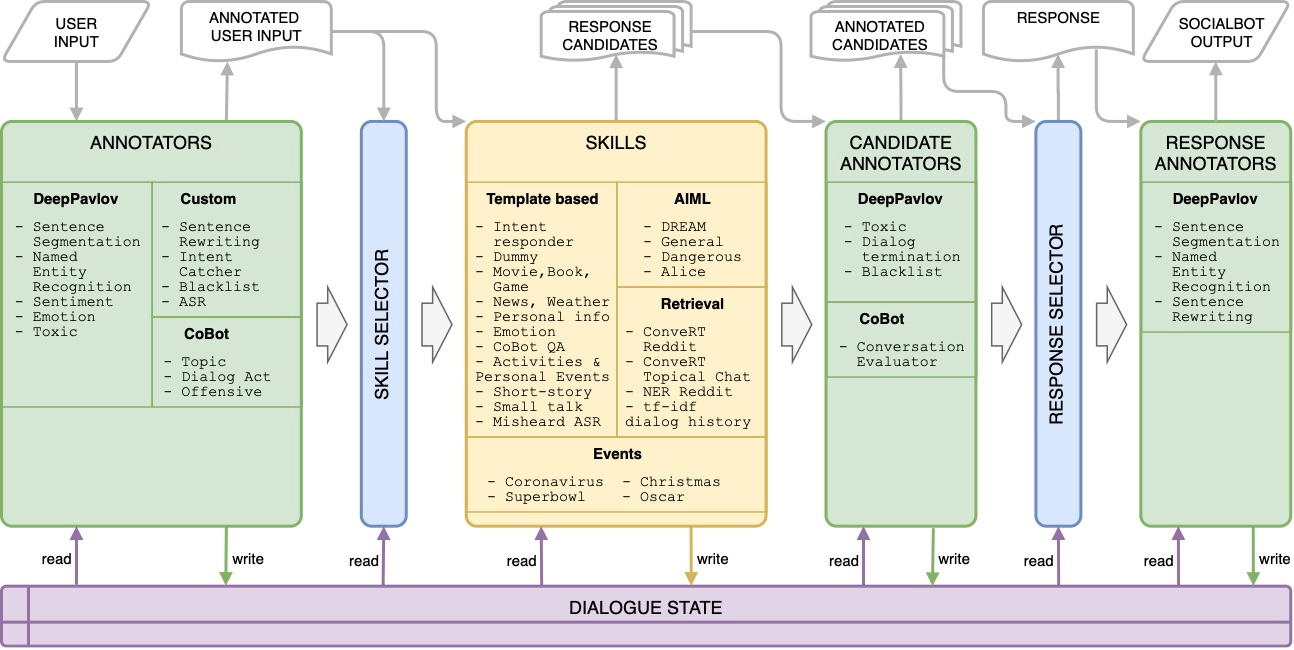
\includegraphics[width=0.8\linewidth]{images/Alexa1_.png} 
\end{frame}

\begin{frame}{Диалоговая платформа DREAM}
    \frametitle{Архитектура диалоговой платформы {DREAM} в конкурсе «Alexa Prize Challenge 4»}
    \centering
    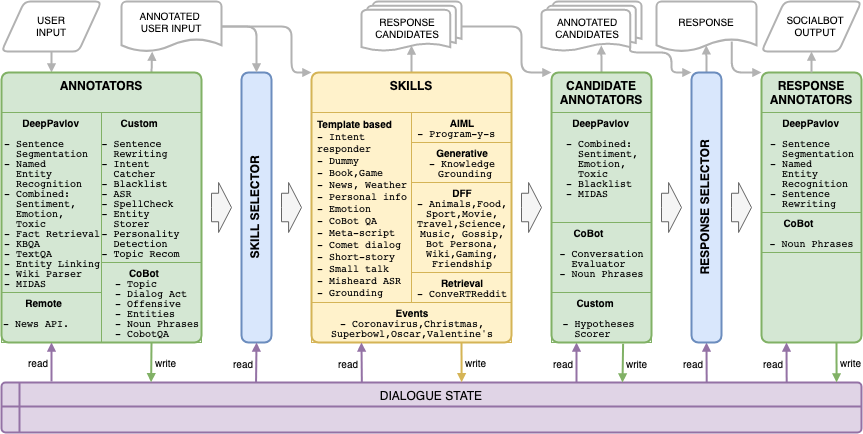
\includegraphics[width=0.8\linewidth]{images/Alexa2_.png} 
\end{frame}

\begin{frame}{Вклад автора в диалоговую платформу DREAM}
\begin{enumerate}
 \item Навыки для обсуждения книг (Book Skill), эмоций (Emotion Skill), сплетен (Gossip Skill, коронавируса (Coronavirus Skill), слухов (Gossip Skill), для обоснования диалога (Grounding Skill), ранжирующий навык TF-IDF (TF-IDF Retrieval), а также генеративный навык, не тестировавшийся на пользователях.
 \item Аннотаторы для классификации эмоций (Emotion Classification), интентов (Intent Catcher), момента остановки диалога (Stop Detect).
 \item Модели для многозадачной классификации (подробнее - в следующих слайдах)
\end{enumerate}
\end{frame}
\begin{frame}{Зачем нужны модели для многозадачной классификации?}
\begin{enumerate}
\item Экономия на вычислительных ресурсах. Стоимость GPU для DREAM во время Alexa Prize 4 до 9000\$/мес.
\item Замена удаленных сервисов от Amazon, т.к они были доступны не всегда.
\end{enumerate}
\end{frame}
\begin{frame}{Модели для многозадачной классификации - с одним линейным слоем}
\begin{enumerate}
\item Замена классификаторов от Amazon (Cobot Topics, Cobot DialogAct Topics, Cobot Conversation Evaluator), чтобы система DREAM могла работать безотносительно политики этой компании.
\item Замена однозадачных классификаторов (Emotion Classification, Sentiment Classification, Toxic Classification) для экономии вычислительных ресурсов.
\end{enumerate}
\end{frame}
\begin{frame}{Модели для многозадачной классификации - с одним линейным слоем}
\begin{table}[htbp]
\caption{Точность на различных задачах для разных типов однозадачных моделей, в сравнении с многозадачными. }
    \scalebox{0.65}{
    \begin{tabular}{|c|c|c|c|c|} 
    \hline
    \multirow{2}{*}{3адача} & \multicolumn{4}{c|}{Модели} \\
    \cline{2-5}
     & \textbf{Однозадачные} & \textbf{6 в 1} & \textbf{3 в 1 (cobot)} & \textbf{3 в 1 (не cobot)}\\ 
    \hline
    cobot topics   & --- & 84 & 82 & --- \\
    \hline
    cobot dialogact topics  & --- & 76 & 78 & --- \\ 
    \hline
    cobot dialogact intents & --- & 69 & 70 & --- \\ 
    \hline
    Эмоции  & 92 & 82 & --- & 85 \\
    \hline
    Тональность & 72 & 60 & --- & 66 \\ 
    \hline
    Токсичность & 92 & 92 & --- & 93\\ 
    \hline
    \end{tabular}}
\end{table}
\end{frame}

\begin{frame}{Модели с одним линейным слоем - замена сервисов Amazon}
Также модели с одним линейным слоем применяются для замены модуля оценки диалога от Amazon (Cobot Conversation Evaluator). СКО = 0.31.
\end{frame}

\begin{frame}{Модели для многозадачной классификации - трансформер-инвариантные}
Добавлены новые задачи - 
\begin{enumerate}
    \item Тематическая классификация DeepPavlov Topics.
    \item Классификация фактоидности от YAHOO
    \item Классификация интентов от MIDAS
\end{enumerate}
Также улучшена предобработка наборов данных для остальных задач, или же была произведена замена наборов данных.
\end{frame}
\begin{frame}{Трансформер-инвариантные модели - результаты}
\begin{table}[htbp]
\caption{Точность/взвешенный-F1) для оценки моделей в экспериментах с трансформер-инвариантными моделями. Для не-Коботовских задач при оценке используются оригинальные тестовые наборы данных, для коботовских -- тестовая часть разбиения данных. Как distilbert обозначается модель \textit{distilbert-base-uncased}, как bert модель \textit{bert-base-uncased}. «С историей» означает использование диалоговой истории только в задаче MIDAS, «Без истории» означает, что деалоговая история не использовалась ни в одной задаче «Размер» означает размер обучающей выборки. Режим S означает, что обучались однозадачные модели, M означает, что обучалась многозадачная модель.}
\scalebox{0.6}{
\begin{tabular}{|c||c|c|c|c|c|c|} \hline

Задача & Размер &\begin{tabular}[c]{@{}l@{}}distilbert, S\\с историей\end{tabular} & \begin{tabular}[c]{@{}l@{}}distilbert, M\\с историей\end{tabular}  & \begin{tabular}[c]{@{}l@{}}distilbert, M\\без истории\end{tabular} & \begin{tabular}[c]{@{}l@{}}bert, S\\с историей\end{tabular} & \begin{tabular}[c]{@{}l@{}}bert, M\\с историей\end{tabular}\\ \hline \hline
       
Эмоции              & 39.5k & 70.47 & 68.18 & 67.59       & 71.48 & 67.27 \\ \hline
Токсичность            & 162k & 94.53 & 93.84  & 93.86        & 94.54 & 93.94 \\ \hline
Тональность            & 94k  & 74.75 & 72.55 & 72.22          & 75.95 & 75.65 \\ \hline
Интенты MIDAS          & 7.1k & 80.53 & 72.73 & 73.69 & 82.3  & 77.01 \\ \hline
DeepPavlov Topics & 1.8M & 87.48 & 86.98  & 87.01         & 88.09  & 87.43 \\ \hline
cobot topics ~                  & 216k & 79.88 & 77.31 & 77.45        & 80.68 & 78.21 \\ \hline
\begin{tabular}[c]{@{}l@{}}cobot dialogact\\ topics \end{tabular}            & 127k & 76.81 & 76.92 & 76.8          & 77.02 & 76.86 \\ \hline
\begin{tabular}[c]{@{}l@{}}cobot dialogact \\intents \end{tabular}           & 318k & 77.07  & 76.83 & 76.65        & 77.28 & 76.96 \\ \hline
Средее для 9 задач                   & 2.76M & 80.36    & 78.48 & 78.36        & 81.31  & 79.3 \\ \hline
\begin{tabular}[c]{@{}l@{}} Видеопамяти \\ использовано, Мб    \end{tabular}            &    & 2418*9=21762 & 2420     & 2420             & 3499*9=31491 & 3501    \\ \hline
\end{tabular}
}
\end{table}
\end{frame}


\begin{frame}{Модели для многозадачной классификации - что не сработало}
\begin{enumerate}
\item Использовался PAL-BERT, но был отброшен, т.к модель не трансформер-агностична.
\item Использовалаь псевдоразметка данных, но была отброшена, т.к процедура вносила слишком сильные искажения в распределение классов.
\end{enumerate}
\end{frame}


\begin{frame}{Научная новизна}
\begin{itemize}
  \item {Выявлены закономерности переноса знаний при псевдоразметке данных для многозадачных нейросетевых моделей с одним линейным слоем.}
  \item {Выявлены закономерности переноса знаний в трансформер-инвариантных многозадачных нейросетевых моделях между различными диалоговыми задачами и языками. Была получена оценка зависимости этого переноса от размера обучающей выборки. Была проверена также справедливость выводов о межъязыковом переносе для однозадачных моделей.}
  \item {Получена оценка зависимости межъязыкового переноса знаний на разговорных данных в многоязычных нейросетевых моделях от размера предобучающей выборки и генеалогической близости языков к языку дообучения.}
\end{itemize}    
\end{frame}

\begin{frame}{Научная новизна}
\begin{itemize}
  \item {Разработана диалоговая платформа DREAM, задачи которой пригодны для изучения прикладного применения многозадачных нейросетевых моделей.}
  \item {Рассмотренные в диссертации многозадачные нейросетевые архитектуры были интегрированы в диалоговую платформу DREAM, была оценена их применимость и был проведен их сравнительный анализ на основе опыта применения. На основании этого анализа была произведена также интеграция в библиотеку DeepPavlov, находящуюся в открытом доступе.}
\end{itemize}    
\end{frame}




\begin{frame}
    \frametitle{Положения, выносимые на защиту}
    \begin{itemize}
  \item {Псевдоразметка данных при помощи однозадачных моделей улучшает метрики многозадачных моделей. При этом объединение классов оправдывает себя только для задач, достаточно сильно похожих друг на друга.}
  \item {Для достаточно малых данных многозадачные трансформер-инвариантные модели начинают превосходить по своей средней точности однозадачные, в особенности -- за счет задач с наименьшим объемом данных. При этом для таких многоязычных моделей наблюдается также перенос знаний с английского языка на русский в рамках одной задачи, и чем меньше русскоязычных данных, тем сильнее выражен перенос. Эта закономерность справедлива и для однозадачных моделей.}
  \item {Для многоязычных нейросетевых моделей качество переноса знаний на разные языки на тематических данных сильно коррелирует с размером предобучающей выборки для каждого языка, но при этом не коррелирует с генеалогической близостью этого языка к языку дообучения.}
    \end{itemize}
\end{frame}

\begin{frame}{Практическая значимость}
\begin{enumerate}
   \item Впервые в России была создана диалоговая платформа мирового уровня, вышедшая в полуфинал престижных мировых конкурсов Alexa Prize 3 и Alexa Prize 4 (в конкурсах было 10 и 9 участников соответственно, из более чем 300 кандидатов). Эта диалоговая платформа имеет полностью открытый код, что дает возможность легкого переиспользования любой части проделанной над ней работы. Были также разработаны сценарные навыки для этой платформы.
   \item В данной диалоговой платформе были применены многозадачные нейросетевые модели: многозадачная нейросетевая модель с одним линейным слоем, многозадачная нейросетевая модель на основе архитектуры PAL-BERT и многозадачная трансформер-инвариантная нейросетевая модель.
   \item Программный код для реализации многозадачной трансформер-инвариантной нейросетевой модели встроен в библиотеку DeepPavlov, имеющую более 500000 скачиваний на март 2023 года.
\end{enumerate}    
\end{frame}


\begin{frame}{Основные публикации}
 Основные результаты по теме диссертации изложены в 9~публикациях,{1} из которых издано в журналах, рекомендованных ВАК, {1} в~периодических научных журналах, индексируемых Web of~Science и Scopus (еще 2 - принято в такие журналы и готовится к публикации), {4} в~тезисах докладов.\footnote{Цифры будут уточнены после принятия всех статей.} Получен также 1 патент.
\end{frame}
\begin{frame}{Основные публикации}
\begin{enumerate}
 \item Karpov, D. Data pseudo-labeling while adapting BERT for multitask
approaches  / D. Karpov, M. Burtsev // Komp’juternaja
Lingvistika i Intellektual’nye Tehnologii. — 2021. — С. 358—366.
\item  Karpov, D. Knowledge Transfer in the Multi-task Transformer-agnostic
Models On Conversational Tasks (готовится к публикации) /
D. Karpov, V. Konovalov // Proceedings of the International Conference
«Dialogue 2023». — 2023.
\item Karpov, D. Multi-task Transformer-Agnostic Models For Conversational
Tasks (на рецензировании) / D. Karpov, V. Konovalov //
Proceedings of InterSpeech 2023. — 2023.
\item Karpov, D. Monolingual and Cross-Lingual Knowledge Transfer for
Topic Classification (готовится к публикации)/ D. Karpov,
M. Burtsev // Proceedings of AINL 2023. — 2023.
\end{enumerate}
\end{frame}

\begin{frame}{Основные публикации}
\begin{enumerate}
\item DREAM technical report for the Alexa Prize 2019 / Y. Kuratov
[и др.] // 3rd Proc. Alexa Prize. — 2019.
\item DREAM technical report for the Alexa Prize 4  / D. Baymurzina
[и др.] // 4th Proc. Alexa Prize. — 2021.
\item Юсупов И.Ф. и Баймурзина Д.Р. и Кузнецов Д.П. и Чернявский Д.В. и Дмитриевский А. и Ермакова Е.С. и Игнатов Ф.С. и Карпов Д.А. и Корнев Д.А. и Ли Т.А. и Пугин П.Ю. и Бурцев М.С., К. Ю. и. Диалоговая система DREAM в конкурсе Alexa
Prize Challenge 2019 // Труды Московского физико-технического
института. — 2021. — Т. 13, 3 (51). — С. 62—89
\item DeepPavlov Dream: Platform for Building Multiskill Generative Assistants / Dilyara Zharikova, Daniel Kornev, Fedor Ignatov, Maxim Talimanchuk, Dmitry Evseev, Ksenya Petukhova, Veronika Smilga, Dmitry Karpov, Yana Shishkina, Dmitry Kosenko and Mikhail Burtsev / Proceedings of the ACL Systems Demo, 2023
\end{enumerate}
\end{frame}
\begin{frame}{Основные публикации}
\begin{enumerate}
\item Разработка диалоговой системы с интеграцией профиля лично­
сти  / Д. Болотин [и др.] //. 5th International Conference
on Engineering and Telecommunication EnT—MIPT 2018. — MIPT,
2019. — URL: http://2019.en-t.info/old/articles/ent2018-thesis.pdf ;
Конференция проходила 15-16 декабря 2018 года. Место проведения:
Москва/Долгопрудный/«Физтехпарк».
\item Свидетельство о депонировании, Texter ocr-cv-nlp-microservice / В. Дуплякин [и др.]. — 2021.
\end{enumerate}    
\end{frame}


\begin{frame}{Практическая значимость}
\begin{enumerate}
   \item Впервые в России была создана диалоговая платформа мирового уровня, вышедшая в полуфинал престижных мировых конкурсов Alexa Prize 3 и Alexa Prize 4 (в конкурсах было 10 и 9 участников соответственно, из более чем 300 кандидатов). Эта диалоговая платформа имеет полностью открытый код, что дает возможность легкого переиспользования любой части проделанной над ней работы. Были также разработаны сценарные навыки для этой платформы.
   \item В данной диалоговой платформе были применены многозадачные нейросетевые модели: многозадачная нейросетевая модель с одним линейным слоем, многозадачная нейросетевая модель на основе архитектуры PAL-BERT и многозадачная трансформер-инвариантная нейросетевая модель.
   \item Программный код для реализации многозадачной трансформер-инвариантной нейросетевой модели встроен в библиотеку DeepPavlov, имеющую более 500000 скачиваний на март 2023 года.
\end{enumerate}    
\end{frame}

\begin{frame}{Спасибо за внимание}
\end{frame}